
%% RoboCupRescue_TDP.tex
%% V0.1
%% 2018/10/22
%% by Soeren Schwertfeger
%% robotics.shanghaitech.edu.cn
%%
%% Based on bare_jtnl.tex
%%
%% (requires IEEEtran.cls version 1.8b or later) with an IEEE
%% journal paper.
%%


%%*************************************************************************
%% Legal Notice:
%% This code is offered as-is without any warranty either expressed or
%% implied; without even the implied warranty of MERCHANTABILITY or
%% FITNESS FOR A PARTICULAR PURPOSE! 
%% User assumes all risk.
%% In no event shall the IEEE or any contributor to this code be liable for
%% any damages or losses, including, but not limited to, incidental,
%% consequential, or any other damages, resulting from the use or misuse
%% of any information contained here.
%%
%% All comments are the opinions of their respective authors and are not
%% necessarily endorsed by the IEEE.
%%
%% This work is distributed under the LaTeX Project Public License (LPPL)
%% ( http://www.latex-project.org/ ) version 1.3, and may be freely used,
%% distributed and modified. A copy of the LPPL, version 1.3, is included
%% in the base LaTeX documentation of all distributions of LaTeX released
%% 2003/12/01 or later.
%% Retain all contribution notices and credits.
%% ** Modified files should be clearly indicated as such, including  **
%% ** renaming them and changing author support contact information. **
%%*************************************************************************


% *** Authors should verify (and, if needed, correct) their LaTeX system  ***
% *** with the testflow diagnostic prior to trusting their LaTeX platform ***
% *** with production work. The IEEE's font choices and paper sizes can   ***
% *** trigger bugs that do not appear when using other class files.       ***                          ***
% The testflow support page is at:
% http://www.michaelshell.org/tex/testflow/



\documentclass[journal]{IEEEtran}
%
% If IEEEtran.cls has not been installed into the LaTeX system files,
% manually specify the path to it like:
% \documentclass[journal]{../sty/IEEEtran}


% Some very useful LaTeX packages include:
% (uncomment the ones you want to load)


% *** MISC UTILITY PACKAGES ***
%
%\usepackage{ifpdf}
% Heiko Oberdiek's ifpdf.sty is very useful if you need conditional
% compilation based on whether the output is pdf or dvi.
% usage:
% \ifpdf
%   % pdf code
% \else
%   % dvi code
% \fi
% The latest version of ifpdf.sty can be obtained from:
% http://www.ctan.org/pkg/ifpdf
% Also, note that IEEEtran.cls V1.7 and later provides a builtin
% \ifCLASSINFOpdf conditional that works the same way.
% When switching from latex to pdflatex and vice-versa, the compiler may
% have to be run twice to clear warning/error messages.






% *** CITATION PACKAGES ***
%
%\usepackage{cite}
% cite.sty was written by Donald Arseneau
% V1.6 and later of IEEEtran pre-defines the format of the cite.sty package
% \cite{} output to follow that of the IEEE. Loading the cite package will
% result in citation numbers being automatically sorted and properly
% "compressed/ranged". e.g., [1], [9], [2], [7], [5], [6] without using
% cite.sty will become [1], [2], [5]--[7], [9] using cite.sty. cite.sty's
% \cite will automatically add leading space, if needed. Use cite.sty's
% noadjust option (cite.sty V3.8 and later) if you want to turn this off
% such as if a citation ever needs to be enclosed in parenthesis.
% cite.sty is already installed on most LaTeX systems. Be sure and use
% version 5.0 (2009-03-20) and later if using hyperref.sty.
% The latest version can be obtained at:
% http://www.ctan.org/pkg/cite
% The documentation is contained in the cite.sty file itself.


\usepackage[pdfborder=0 0 0,colorlinks=true,urlcolor=blue,citecolor=blue, linkcolor=blue]{hyperref}



% *** GRAPHICS RELATED PACKAGES ***
%
\ifCLASSINFOpdf
  \usepackage[pdftex]{graphicx}
  % declare the path(s) where your graphic files are
  % \graphicspath{{../pdf/}{../jpeg/}}
  % and their extensions so you won't have to specify these with
  % every instance of \includegraphics
  % \DeclareGraphicsExtensions{.pdf,.jpeg,.png}
\else
  % or other class option (dvipsone, dvipdf, if not using dvips). graphicx
  % will default to the driver specified in the system graphics.cfg if no
  % driver is specified.
  % \usepackage[dvips]{graphicx}
  % declare the path(s) where your graphic files are
  % \graphicspath{{../eps/}}
  % and their extensions so you won't have to specify these with
  % every instance of \includegraphics
  % \DeclareGraphicsExtensions{.eps}
\fi
% graphicx was written by David Carlisle and Sebastian Rahtz. It is
% required if you want graphics, photos, etc. graphicx.sty is already
% installed on most LaTeX systems. The latest version and documentation
% can be obtained at: 
% http://www.ctan.org/pkg/graphicx
% Another good source of documentation is "Using Imported Graphics in
% LaTeX2e" by Keith Reckdahl which can be found at:
% http://www.ctan.org/pkg/epslatex
%
% latex, and pdflatex in dvi mode, support graphics in encapsulated
% postscript (.eps) format. pdflatex in pdf mode supports graphics
% in .pdf, .jpeg, .png and .mps (metapost) formats. Users should ensure
% that all non-photo figures use a vector format (.eps, .pdf, .mps) and
% not a bitmapped formats (.jpeg, .png). The IEEE frowns on bitmapped formats
% which can result in "jaggedy"/blurry rendering of lines and letters as
% well as large increases in file sizes.
%
% You can find documentation about the pdfTeX application at:
% http://www.tug.org/applications/pdftex





% *** MATH PACKAGES ***
%
%\usepackage{amsmath}
% A popular package from the American Mathematical Society that provides
% many useful and powerful commands for dealing with mathematics.
%
% Note that the amsmath package sets \interdisplaylinepenalty to 10000
% thus preventing page breaks from occurring within multiline equations. Use:
%\interdisplaylinepenalty=2500
% after loading amsmath to restore such page breaks as IEEEtran.cls normally
% does. amsmath.sty is already installed on most LaTeX systems. The latest
% version and documentation can be obtained at:
% http://www.ctan.org/pkg/amsmath





% *** SPECIALIZED LIST PACKAGES ***
%
%\usepackage{algorithmic}
% algorithmic.sty was written by Peter Williams and Rogerio Brito.
% This package provides an algorithmic environment fo describing algorithms.
% You can use the algorithmic environment in-text or within a figure
% environment to provide for a floating algorithm. Do NOT use the algorithm
% floating environment provided by algorithm.sty (by the same authors) or
% algorithm2e.sty (by Christophe Fiorio) as the IEEE does not use dedicated
% algorithm float types and packages that provide these will not provide
% correct IEEE style captions. The latest version and documentation of
% algorithmic.sty can be obtained at:
% http://www.ctan.org/pkg/algorithms
% Also of interest may be the (relatively newer and more customizable)
% algorithmicx.sty package by Szasz Janos:
% http://www.ctan.org/pkg/algorithmicx




% *** ALIGNMENT PACKAGES ***
%
%\usepackage{array}
% Frank Mittelbach's and David Carlisle's array.sty patches and improves
% the standard LaTeX2e array and tabular environments to provide better
% appearance and additional user controls. As the default LaTeX2e table
% generation code is lacking to the point of almost being broken with
% respect to the quality of the end results, all users are strongly
% advised to use an enhanced (at the very least that provided by array.sty)
% set of table tools. array.sty is already installed on most systems. The
% latest version and documentation can be obtained at:
% http://www.ctan.org/pkg/array


% IEEEtran contains the IEEEeqnarray family of commands that can be used to
% generate multiline equations as well as matrices, tables, etc., of high
% quality.




% *** SUBFIGURE PACKAGES ***
%\ifCLASSOPTIONcompsoc
%  \usepackage[caption=false,font=normalsize,labelfont=sf,textfont=sf]{subfig}
%\else
%  \usepackage[caption=false,font=footnotesize]{subfig}
%\fi
% subfig.sty, written by Steven Douglas Cochran, is the modern replacement
% for subfigure.sty, the latter of which is no longer maintained and is
% incompatible with some LaTeX packages including fixltx2e. However,
% subfig.sty requires and automatically loads Axel Sommerfeldt's caption.sty
% which will override IEEEtran.cls' handling of captions and this will result
% in non-IEEE style figure/table captions. To prevent this problem, be sure
% and invoke subfig.sty's "caption=false" package option (available since
% subfig.sty version 1.3, 2005/06/28) as this is will preserve IEEEtran.cls
% handling of captions.
% Note that the Computer Society format requires a larger sans serif font
% than the serif footnote size font used in traditional IEEE formatting
% and thus the need to invoke different subfig.sty package options depending
% on whether compsoc mode has been enabled.
%
% The latest version and documentation of subfig.sty can be obtained at:
% http://www.ctan.org/pkg/subfig




% *** FLOAT PACKAGES ***
%
%\usepackage{fixltx2e}
% fixltx2e, the successor to the earlier fix2col.sty, was written by
% Frank Mittelbach and David Carlisle. This package corrects a few problems
% in the LaTeX2e kernel, the most notable of which is that in current
% LaTeX2e releases, the ordering of single and double column floats is not
% guaranteed to be preserved. Thus, an unpatched LaTeX2e can allow a
% single column figure to be placed prior to an earlier double column
% figure.
% Be aware that LaTeX2e kernels dated 2015 and later have fixltx2e.sty's
% corrections already built into the system in which case a warning will
% be issued if an attempt is made to load fixltx2e.sty as it is no longer
% needed.
% The latest version and documentation can be found at:
% http://www.ctan.org/pkg/fixltx2e


%\usepackage{stfloats}
% stfloats.sty was written by Sigitas Tolusis. This package gives LaTeX2e
% the ability to do double column floats at the bottom of the page as well
% as the top. (e.g., "\begin{figure*}[!b]" is not normally possible in
% LaTeX2e). It also provides a command:
%\fnbelowfloat
% to enable the placement of footnotes below bottom floats (the standard
% LaTeX2e kernel puts them above bottom floats). This is an invasive package
% which rewrites many portions of the LaTeX2e float routines. It may not work
% with other packages that modify the LaTeX2e float routines. The latest
% version and documentation can be obtained at:
% http://www.ctan.org/pkg/stfloats
% Do not use the stfloats baselinefloat ability as the IEEE does not allow
% \baselineskip to stretch. Authors submitting work to the IEEE should note
% that the IEEE rarely uses double column equations and that authors should try
% to avoid such use. Do not be tempted to use the cuted.sty or midfloat.sty
% packages (also by Sigitas Tolusis) as the IEEE does not format its papers in
% such ways.
% Do not attempt to use stfloats with fixltx2e as they are incompatible.
% Instead, use Morten Hogholm'a dblfloatfix which combines the features
% of both fixltx2e and stfloats:
%
% \usepackage{dblfloatfix}
% The latest version can be found at:
% http://www.ctan.org/pkg/dblfloatfix




%\ifCLASSOPTIONcaptionsoff
%  \usepackage[nomarkers]{endfloat}
% \let\MYoriglatexcaption\caption
% \renewcommand{\caption}[2][\relax]{\MYoriglatexcaption[#2]{#2}}
%\fi
% endfloat.sty was written by James Darrell McCauley, Jeff Goldberg and 
% Axel Sommerfeldt. This package may be useful when used in conjunction with 
% IEEEtran.cls'  captionsoff option. Some IEEE journals/societies require that
% submissions have lists of figures/tables at the end of the paper and that
% figures/tables without any captions are placed on a page by themselves at
% the end of the document. If needed, the draftcls IEEEtran class option or
% \CLASSINPUTbaselinestretch interface can be used to increase the line
% spacing as well. Be sure and use the nomarkers option of endfloat to
% prevent endfloat from "marking" where the figures would have been placed
% in the text. The two hack lines of code above are a slight modification of
% that suggested by in the endfloat docs (section 8.4.1) to ensure that
% the full captions always appear in the list of figures/tables - even if
% the user used the short optional argument of \caption[]{}.
% IEEE papers do not typically make use of \caption[]'s optional argument,
% so this should not be an issue. A similar trick can be used to disable
% captions of packages such as subfig.sty that lack options to turn off
% the subcaptions:
% For subfig.sty:
% \let\MYorigsubfloat\subfloat
% \renewcommand{\subfloat}[2][\relax]{\MYorigsubfloat[]{#2}}
% However, the above trick will not work if both optional arguments of
% the \subfloat command are used. Furthermore, there needs to be a
% description of each subfigure *somewhere* and endfloat does not add
% subfigure captions to its list of figures. Thus, the best approach is to
% avoid the use of subfigure captions (many IEEE journals avoid them anyway)
% and instead reference/explain all the subfigures within the main caption.
% The latest version of endfloat.sty and its documentation can obtained at:
% http://www.ctan.org/pkg/endfloat
%
% The IEEEtran \ifCLASSOPTIONcaptionsoff conditional can also be used
% later in the document, say, to conditionally put the References on a 
% page by themselves.


% *** PDF, URL AND HYPERLINK PACKAGES ***
%
\usepackage{url}
% url.sty was written by Donald Arseneau. It provides better support for
% handling and breaking URLs. url.sty is already installed on most LaTeX
% systems. The latest version and documentation can be obtained at:
% http://www.ctan.org/pkg/url
% Basically, \url{my_url_here}.




% *** Do not adjust lengths that control margins, column widths, etc. ***
% *** Do not use packages that alter fonts (such as pslatex).         ***
% There should be no need to do such things with IEEEtran.cls V1.6 and later.
% (Unless specifically asked to do so by the journal or conference you plan
% to submit to, of course. )


% correct bad hyphenation here
\hyphenation{op-tical net-works semi-conduc-tor}


%
% Specify the venure for this TDP, e.g.:
%
% for the world cup just the year:
% \newcommand{\TDPyear}{2016~}
%
% for regional competitions the regional name, too
% \newcommand{\TDPyear}{German Open 2016~}

\newcommand{\TDPvenue}{2019~}

\begin{document}
%
% paper title
% Titles are generally capitalized except for words such as a, an, and, as,
% at, but, by, for, in, nor, of, on, or, the, to and up, which are usually
% not capitalized unless they are the first or last word of the title.
% Linebreaks \\ can be used within to get better formatting as desired.
% Do not put math or special symbols in the title.
\title{RoboCup Rescue \TDPvenue Team Description Paper \\
 Club Capra}

%
% author names - no IEEE memberships
% only the authors for this TDP - not necessarily all team members!
%

\author{Alexandre~Francoeur,
        Ludovic~Vanasse,
        and~Marc-Olivier~B\'elisle% <-this % stops a space
\thanks{A. Francoeur, L. Vanasse and M-O. B\'elisle are with the scientific student club Capra, \'Ecole de technologie sup\'erieure, Montr\'eal, e-mail: capra@clubcapra.com.}% <-this % stops a space
%\thanks{J. Doe and J. Doe are with Anonymous University.}% <-this % stops a space
%\thanks{Manuscript received April 19, 2005; revised August 26, 2015.} no need for received dates!?
}


% note the % following the last \IEEEmembership and also \thanks - 
% these prevent an unwanted space from occurring between the last author name
% and the end of the author line. i.e., if you had this:
% 
% \author{....lastname \thanks{...} \thanks{...} }
%                     ^------------^------------^----Do not want these spaces!
%
% a space would be appended to the last name and could cause every name on that
% line to be shifted left slightly. This is one of those "LaTeX things". For
% instance, "\textbf{A} \textbf{B}" will typeset as "A B" not "AB". To get
% "AB" then you have to do: "\textbf{A}\textbf{B}"
% \thanks is no different in this regard, so shield the last } of each \thanks
% that ends a line with a % and do not let a space in before the next \thanks.
% Spaces after \IEEEmembership other than the last one are OK (and needed) as
% you are supposed to have spaces between the names. For what it is worth,
% this is a minor point as most people would not even notice if the said evil
% space somehow managed to creep in.



% The paper headers
% \markboth{Journal of \LaTeX\ Class Files,~Vol.~14, No.~8, August~2015}%
% {Shell \MakeLowercase{\textit{et al.}}: Bare Demo of IEEEtran.cls for IEEE Journals}
\markboth{RoboCup Rescue \TDPvenue TDP Collection}%
{Francoeur \MakeLowercase{\textit{et al.}}: Club Capra}
% The only time the second header will appear is for the odd numbered pages
% after the title page when using the twoside option.
% 
% *** Note that you probably will NOT want to include the author's ***
% *** name in the headers of peer review papers.                   ***
% You can use \ifCLASSOPTIONpeerreview for conditional compilation here if
% you desire.




% If you want to put a publisher's ID mark on the page you can do it like
% this:
%\IEEEpubid{0000--0000/00\$00.00~\copyright~2015 IEEE}
% Remember, if you use this you must call \IEEEpubidadjcol in the second
% column for its text to clear the IEEEpubid mark.



% use for special paper notices
%\IEEEspecialpapernotice{(Invited Paper)}




% make the title area
\maketitle



% As a general rule, do not put math, special symbols or citations
% in the abstract or keywords.

\begin{flushleft}
\textbf{Info}\\
\hspace{10pt} Team Name: \hfill Club Capra\\
\hspace{10pt} Team Institution: \hfill \'Ecole de technologie sup\'erieure\\
\hspace{10pt} Team Leader: \hfill Alexandre Francoeur\\
\hspace{10pt} Team URL: \hfill \url{https://clubcapra.com}
\\
\vspace{5pt}
\hspace{10pt} RoboCup Rescue \TDPvenue TDP collection: \\
\hfill \url{https://robocup-rescue.github.io/team_description_papers/}
\end{flushleft}

\begin{abstract}
The abstract goes here. Do not describe RoboCup Rescue in detail - concentrate on your robots, their main capabilities and what sets them apart from the competitors.
\end{abstract}

% RoboCup Rescue and Team Description Paper have to be the frist two keywords. You can select up to three more keywords.
\begin{IEEEkeywords}
RoboCup Rescue, Team Description Paper, Search and Rescue Robots, Robotics in Hazardous Fields.
\end{IEEEkeywords}






% For peer review papers, you can put extra information on the cover
% page as needed:
% \ifCLASSOPTIONpeerreview
% \begin{center} \bfseries EDICS Category: 3-BBND \end{center}
% \fi
%
% For peerreview papers, this IEEEtran command inserts a page break and
% creates the second title. It will be ignored for other modes.
\IEEEpeerreviewmaketitle





\section{Introduction}
% The very first letter is a 2 line initial drop letter followed
% by the rest of the first word in caps.
% 
% form to use if the first word consists of a single letter:
% \IEEEPARstart{A}{demo} file is ....
% 
% form to use if you need the single drop letter followed by
% normal text (unknown if ever used by the IEEE):
% \IEEEPARstart{A}{}demo file is ....
% 
% Some journals put the first two words in caps:
% \IEEEPARstart{T}{his demo} file is ....
% 
% Here we have the typical use of a "T" for an initial drop letter
% and "HIS" in caps to complete the first word.
% \IEEEPARstart{T}{his} demo file is intended to serve as a ``starter file''
% for IEEE journal papers produced under \LaTeX\ using
% IEEEtran.cls version 1.8b and later.
% You must have at least 2 lines in the paragraph with the drop letter
% (should never be an issue)

\IEEEPARstart{P}{lease} use this Team Description Paper (TDP) template to answer the following questions about your team's approach to designing, fabricating, controlling, and operating your urban search and rescue robot team. We will likely have many more teams interested in participating than we can accommodate, so we will use this paper to initially qualify your team for final registration. We are looking for teams showing solid progress toward a functioning system, particularly innovative approaches, and well formulated (and well described) team strategies.  Timely submittal of this and other documents is also appreciated.


It is very important that you follow this particular template regarding formatting. From 2017 on we plan make the TDPs of all qualified teams publicly available via the webpage \url{https://robocup-rescue.github.io/team_description_papers/} . We understand that at this early date your system is likely not fully realized, so we expect this document to be incomplete in parts.  However, we expect you to articulate at least some ideas in each area outlined below.  The more comprehensive your approach appears, the more favorably it will be reviewed. If you have hardware implemented, please add lots of pictures as you describe your system, and give details regarding the parts themselves (sensors, motors, joysticks, etc).  If you have drawings of your system, please include them. If you have particular team strategies, please describe them. Otherwise, please attempt to describe at least the direction you are going in any given section and what we can expect to see at the competition.  Please also describe how your operator(s) plan to interact with your system.

The TDP is not the place to describe your awesome new approach in all details with experiments that proof the performance, etc. This should go into an extra paper. Anyways be sure to cite all your relevant publications and also the according publications of other researchers, for example \cite{Sheh2016RoboCupRescue, sheh2011robocuprescue, lorenz2018robocup, Kohlbrecher_community_ssrr_2012, PellenzMappingAndMapScoring2008, sheh2012advancing, jacoff2012robocup, SSRR11-FiducialMapMetric, SSRR07-JacobsAutonomy}... The TDP is an overview paper to show how the system performs as a whole. The introduction should give an overview of your systems and your approach to RoboCup Rescue.

\begin{figure}[!t]
\centering
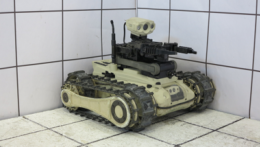
\includegraphics[width=\linewidth]{figs/booth}
\caption{Photo of your robot. Should ideally be located in a corner with lines 10cm apart (at least on the ground). Take the photo from an angle such that front, side and top are visible. This photo should appear on the first page of your document exactly where it is placed in the template! If you have other robots or an unusual operator station add those in extra figures.}
\label{fig:robotPhoto}
\end{figure}


\subsection{Submission}
If you are a) accepted for the RoboCup Rescue competition, b) payed the registration fees AND c) participated in the event we will to publish your TDP on the webpage. 

Please do not include any of the TDP template preparation instructions in your TDP ;)

\subsection{Improvements over Previous Contributions}
If you have previously participated at RoboCup Rescue, describe how your system differs and improves from your previous entry. 

\section{System Description}
Use this section to describe your overall system. Depending on the emphasis of your team the different subsections can be of different lengths. Nevertheless please be as detailed as possible. The advantages are:

\begin{itemize}
 \item Get qualified for RoboCup Rescue by having a detailed system description.
 \item Document your teams approach.
 \item Allow a comparison of your team with other teams.
 \item Allow a comparison between different years of RoboCup and thus (hopefully) a documentation of the improvements through the years.
 \item Allow other and especially new teams to kick-start their research by copying your system.
\end{itemize}

\subsection{Hardware}
Document the hardware of your system. This can be very brief if you bought the robot (in this case mention the major modifications). The first image of this document (should also appear on the first page) should be a photo of your real robot - see Figure \ref{fig:robotPhoto}.

Refer to the Tables \ref{tab:SystemRobot1} and following as well as Table \ref{tab:HardwareList} in the Appendix - there is no need to document part here in detail if it is sufficient to know that it is used from the tables. Please also share your CAD drawings or electronics plans with the community! Do so by adding a big picture to the appending AND by providing the files in a commonly used format as ancillary files \url{http://arxiv.org/help/ancillary_files}.

Explain your approach regarding those topics - create relevant subsubsections as needed:
\begin{itemize}
  \item Locomotion
  \item Power (Batteries)
  \item Electronics, including micro-controllers, etc.
  \item Manipulation/ directed perception
  \item Sensors
  \item Computation (high performance for autonomy, etc.)
  \item Communication is covered in its own subsection - mention the regarding hardware and software there.
  \item Others...
\end{itemize}
\subsection{Software}
Refer to Table \ref{tab:SoftwareList} in the Appendix.

Explain how your software works. Create relevant subsubsections as needed. You might want to explain:
\begin{itemize}
  \item low level control
  \item communication protocol (video, commands, data)
  \item localization
  \item mapping
  \item autonomy
  \item victim detection
  \item path planning
  \item navigation
  \item arm control
  \item arm planning
  \item ...
\end{itemize} 

\subsection{Communication}
Please use this section to describe your plan for communicating with your robots (passive tether, active tether, radio, etc.)  Double check the rules regarding restrictions and rules for the radio! See \url{https://www.robocup.org/leagues/10}.

Report about your wifi hardware in detail. Tell us the vendor and model of your hardware - access point and antennas. Describe which protocol your hardware is working with. Let us know what is the maximum power your hardware supports and what is the power-setting you will be using during the competition.  Tell us the gain of your antennas. Tell us the SSID you will be using (typically it should be "RRL\_teamname"). 
\subsection{Human-Robot Interface}
Explain how your robot is controlled. What does the operator see? In which ways can he interact with the robot? Also describe how a potential user should be trained and how you trained the operator for your team.

\section{Application}

% This section covers the practical aspects of your system...

\subsection{Set-up and Break-Down}
Please use this section to describe your plan for set-up and break-down of your the robots and the operator station.
\subsection{Mission Strategy}
If not already covered in the Introduction, explain your overall strategy to the RoboCup Rescue Challenge. Also mention what you cannot or don't want to do.
\subsection{Experiments}
Explain how you verify your system. Did you build any standard test methods for testing your robot? What kind of experiments and validations did you do with your hardware/ software/ overall systems? What did you learn?
\subsection{Application in the Field}
Discuss how your system is applicable to the field of search and rescue. Where are its strength and weaknesses? What do you think would be possible to improve in the near and medium future towards using it in real scenarios?


% An example of a floating figure using the graphicx package.
% Note that \label must occur AFTER (or within) \caption.
% For figures, \caption should occur after the \includegraphics.
% Note that IEEEtran v1.7 and later has special internal code that
% is designed to preserve the operation of \label within \caption
% even when the captionsoff option is in effect. However, because
% of issues like this, it may be the safest practice to put all your
% \label just after \caption rather than within \caption{}.
%
% Reminder: the "draftcls" or "draftclsnofoot", not "draft", class
% option should be used if it is desired that the figures are to be
% displayed while in draft mode.
%
%\begin{figure}[!t]
%\centering
%\includegraphics[width=2.5in]{myfigure}
% where an .eps filename suffix will be assumed under latex, 
% and a .pdf suffix will be assumed for pdflatex; or what has been declared
% via \DeclareGraphicsExtensions.
%\caption{Simulation results for the network.}
%\label{fig_sim}
%\end{figure}

% Note that the IEEE typically puts floats only at the top, even when this
% results in a large percentage of a column being occupied by floats.


% An example of a double column floating figure using two subfigures.
% (The subfig.sty package must be loaded for this to work.)
% The subfigure \label commands are set within each subfloat command,
% and the \label for the overall figure must come after \caption.
% \hfil is used as a separator to get equal spacing.
% Watch out that the combined width of all the subfigures on a 
% line do not exceed the text width or a line break will occur.
%
%\begin{figure*}[!t]
%\centering
%\subfloat[Case I]{\includegraphics[width=2.5in]{box}%
%\label{fig_first_case}}
%\hfil
%\subfloat[Case II]{\includegraphics[width=2.5in]{box}%
%\label{fig_second_case}}
%\caption{Simulation results for the network.}
%\label{fig_sim}
%\end{figure*}
%
% Note that often IEEE papers with subfigures do not employ subfigure
% captions (using the optional argument to \subfloat[]), but instead will
% reference/describe all of them (a), (b), etc., within the main caption.
% Be aware that for subfig.sty to generate the (a), (b), etc., subfigure
% labels, the optional argument to \subfloat must be present. If a
% subcaption is not desired, just leave its contents blank,
% e.g., \subfloat[].


% An example of a floating table. Note that, for IEEE style tables, the
% \caption command should come BEFORE the table and, given that table
% captions serve much like titles, are usually capitalized except for words
% such as a, an, and, as, at, but, by, for, in, nor, of, on, or, the, to
% and up, which are usually not capitalized unless they are the first or
% last word of the caption. Table text will default to \footnotesize as
% the IEEE normally uses this smaller font for tables.
% The \label must come after \caption as always.
%
%\begin{table}[!t]
%% increase table row spacing, adjust to taste
%\renewcommand{\arraystretch}{1.3}
% if using array.sty, it might be a good idea to tweak the value of
% \extrarowheight as needed to properly center the text within the cells
%\caption{An Example of a Table}
%\label{table_example}
%\centering
%% Some packages, such as MDW tools, offer better commands for making tables
%% than the plain LaTeX2e tabular which is used here.
%\begin{tabular}{|c||c|}
%\hline
%One & Two\\
%\hline
%Three & Four\\
%\hline
%\end{tabular}
%\end{table}


% Note that the IEEE does not put floats in the very first column
% - or typically anywhere on the first page for that matter. Also,
% in-text middle ("here") positioning is typically not used, but it
% is allowed and encouraged for Computer Society conferences (but
% not Computer Society journals). Most IEEE journals/conferences use
% top floats exclusively. 
% Note that, LaTeX2e, unlike IEEE journals/conferences, places
% footnotes above bottom floats. This can be corrected via the
% \fnbelowfloat command of the stfloats package.
\section{Conclusion}
The conclusion goes here. Brief summary, outlook to the competition, lessens learned from previous competitions, etc.





% if have a single appendix:
%\appendix[Proof of the Zonklar Equations]
% or
%\appendix  % for no appendix heading
% do not use \section anymore after \appendix, only \section*
% is possibly needed

% use appendices with more than one appendix
% then use \section to start each appendix
% you must declare a \section before using any
% \subsection or using \label (\appendices by itself
% starts a section numbered zero.)
%


\appendices

\section{Team members and Their Contributions}
Please use this section to recognize all team members and their technical contributions.  Also note your advisors and sponsors, if you choose. You may want to include links to homepages.

\begin{itemize}
 \item  \href{http://www.nist.gov/el/isd/ms/jacoff.cfm}{Adam Jacoff} \hfill Controller development
 \item \href{http://www.rm.is.tohoku.ac.jp/englishtop/}{Satoshi Tadokoro} \hfill Mechanical design
 \item Robo Hero \hfill SLAM algorithm
\end{itemize}



\section{CAD Drawings}
Put one or two nice views of your CAD drawings (for hardware teams - software teams can delete this section). Keep in mind that you can use \textit{\textbackslash begin\{figure*\}} to display an image in full width.

\section{Lists}
\subsection{Systems List}
For every system (each robot individually robot incl. support, Operator Station) answer the following items. One table per system. Remove entries that do not make sense. If a number is unknown try to estimate it or put a question mark (do not delete the entry if it might be interesting but you don't know the answer).

\begin{table}
\renewcommand{\arraystretch}{1}
 \tabcolsep=0.1cm
\caption{Manipulation System}
\label{tab:SystemRobot1}
\centering
\begin{tabular}{|l|r|}
\hline
Attribute & Value \\ \hline
Name & MoonRobbi \\
Locomotion & tracked \\
System Weight & 23kg \\
Weight including transportation case & 28kg \\
Transportation size & 0.6 x 0.6 x 0.5 m \\
Typical operation size & 0.5 x 0.8  x 0.4 m \\
Unpack and assembly time & 180 min \\
Startup time (off to full operation) & 10 min \\
Power consumption (idle/ typical/ max) & 60 / 200 / 800 W \\
Battery endurance (idle/ normal/ heavy load) & 240 / 120 / 60 min\\
Maximum speed (flat/ outdoor/ rubble pile) & 4 / 1 / - m/s\\
Payload (typical, maximum) & 3/ 10 kg\\
Arm: maximum operation height & 160 cm \\
Arm: payload at full extend & 2kg\\
Support: set of bat. chargers total weight & 2.5kg\\
Support: set of bat. chargers power & 1,200W (100-240V AC)\\
Support: Charge time batteries (80\%/ 100\%) & 90 / 120 min\\
Support: Additional set of batteries weight & 2kg\\
Any other interesting attribute & ?\\
Cost & 5000 USD \\
\hline
\end{tabular}
\end{table}

\begin{table}
\renewcommand{\arraystretch}{1}
 \tabcolsep=0.1cm
\caption{Aerial Vehicle}
\label{tab:SystemRobot2}
\centering
\begin{tabular}{|l|r|}
\hline
Attribute & Value \\ \hline
Name & MoonFly \\
Locomotion & quadcopter \\
System Weight & 3kg \\
Weight including transportation case & 6kg \\
Transportation size & 0.6 x 0.6 x 0.5 m \\
Typical operation size & 0.6 x 0.6  x 0.2 m \\
Unpack and assembly time & 10 min \\
Startup time (off to full operation) & 2 min \\
Power consumption (idle/ typical/ max) & 100 / 150 / 300 W \\
Battery endurance (idle/ normal/ heavy load) & 30 / 20 / 15 min\\
Maximum speed & 12 m/s\\
Payload  & 0.15 kg\\
Any other interesting attribute & ?\\
Cost & 2000 USD \\
\hline
\end{tabular}
\end{table}


\begin{table}
\renewcommand{\arraystretch}{1}
 \tabcolsep=0.1cm
\caption{Operator Station}
\label{tab:SystemOp1}
\centering
\begin{tabular}{|l|r|}
\hline
Attribute & Value \\ \hline
Name & MoonOp \\
System Weight & 3.2kg \\
Weight including transportation case & 4.5kg \\
Transportation size & 0.4 x 0.4 x 0.2 m \\
Typical operation size & 0.4 x 0.4  x 0.4 m \\
Unpack and assembly time & 1 min \\
Startup time (off to full operation) & 1 min \\
Power consumption (idle/ typical/ max) & 60 / 80 / 90 W \\
Battery endurance (idle/ normal/ heavy load) & 10 / 5 / 4 h\\
Any other interesting attribute & ?\\
Cost & 2000 USD \\
\hline
\end{tabular}
\end{table}



\subsection{Hardware Components List}
List all interesting components of your Robots and Operator stations.
Include a hyperref link to the product page if possible - see the examples.

\begin{table}
% increase table row spacing, adjust to taste
\renewcommand{\arraystretch}{1}
 \tabcolsep=0.1cm
\caption{Hardware Components List}
\label{tab:HardwareList}
\centering
\begin{tabular}{|c|c|c|c|}
\hline
Part & Brand \& Model & Unit Price & Num.\\
\hline
Drive motors &  \href{http://www.maxonmotor.com/maxon/view/content/products}{Maxon RE 50 200 W}& CHF 870 & 2 \\
Drive gears &  \href{http://www.maxonmotor.com/maxon/view/content/products}{Planetary Gearhead GP 52}&  & 2 \\
Drive encoder &  \href{http://www.maxonmotor.com/maxon/view/content/products}{ Encoder HEDS 5540}&  & 2 \\ 
Motor drivers &  \href{http://example.com}{ }& ? & 2 \\\hline
DC/DC &  \href{http://example.com}{ }& ? & 1 \\
Battery Management &  \href{http://example.com}{ }& ? & 1 \\
Batteries &  \href{http://example.com}{ }& ? & 1 \\\hline
Micro controller &  \href{http://example.com}{ }& ? & 1 \\
Computing Unit &  \href{http://example.com}{ }& ? & 1 \\\hline
WiFi Adapter &  \href{http://example.com}{ }& ? & 1 \\\hline
IMU &  \href{http://example.com}{ }& ? & 4 \\
Cameras &  \href{http://example.com}{ }& ? & 4 \\
PTZ Camera &  \href{http://example.com}{ }& ? & 1 \\
Infrared Camera &  \href{http://example.com}{ }& ? & 1 \\
LRF &  \href{http://example.com}{ }& ? & 2 \\
CO$_2$ Sensor &  \href{http://example.com}{ }& ? & 1 \\\hline
Battery Chargers &  \href{http://example.com}{ }& ? & 4 \\ \hline
6-axis Robot Arm &  \href{http://example.com}{ }& ? & 1 \\ \hline
Aerial Vehicle &  \href{http://example.com}{ }& ? & 1 \\ \hline
Rugged Operator Laptop &  \href{http://example.com}{ }& ? & 1 \\ 

\hline 
\end{tabular}
\end{table}

\subsection{Software List}
List all relevant software packages you (actually) use!
Include a hyperref link to the software page if possible - see the examples. Include version numbers.

If you are using some advanced algorithms be sure to cite the according papers.

When it is not very obvious explain briefly what the software is used for in usage.

\begin{table}
% increase table row spacing, adjust to taste
\renewcommand{\arraystretch}{1}
 \tabcolsep=0.1cm

\caption{Software List}
\label{tab:SoftwareList}
\centering
\begin{tabular}{|c|c|c|c|}
\hline
Name & Version & License & Usage \\
\hline
 \href{http://www.ubuntu.com}{Ubuntu} & 14.04 & open & \\
 \href{http://www.ros.org}{ROS} & jade & BSD & \\
 \href{http://www.pointclouds.org/}{PCL} \cite{Rusu_ICRA2011_PCL}& 1.7 & BSD & ICP \\
 \href{http://opencv.org/}{OpenCV} \cite{990517, 1038171} & 2.4.8 & BSD & Haar: Victim detection \\
 \href{http://opencv.org/}{OpenCV} \cite{Lee2007LBP} & 2.4.8 & BSD & LBP: Hazmat detection \\
 \href{http://wiki.ros.org/hector_slam}{Hector SLAM} \cite{KohlbrecherMeyerStrykKlingaufFlexibleSlamSystem2011} & 0.3.4 & BSD & 2D SLAM \\
 \href{http://robotics.moon.edu}{Moon 3D Mapping} & 0.8 & GPL & 3D Mapping \\
 \href{}{Proprietary GUI from Moon U.} & 0.7 & closed source & Operator Station \\
 
\hline
\end{tabular}
\end{table}




% use section* for acknowledgment
\section*{Acknowledgment}


The authors would like to thank...


% Can use something like this to put references on a page
% by themselves when using endfloat and the captionsoff option.
\ifCLASSOPTIONcaptionsoff
  \newpage
\fi



% trigger a \newpage just before the given reference
% number - used to balance the columns on the last page
% adjust value as needed - may need to be readjusted if
% the document is modified later
%\IEEEtriggeratref{8}
% The "triggered" command can be changed if desired:
%\IEEEtriggercmd{\enlargethispage{-5in}}

% references section

% can use a bibliography generated by BibTeX as a .bbl file
% BibTeX documentation can be easily obtained at:
% http://mirror.ctan.org/biblio/bibtex/contrib/doc/
% The IEEEtran BibTeX style support page is at:
% http://www.michaelshell.org/tex/ieeetran/bibtex/
\bibliographystyle{IEEEtran}
% argument is your BibTeX string definitions and bibliography database(s)
\bibliography{references}
%
% <OR> manually copy in the resultant .bbl file
% set second argument of \begin to the number of references
% (used to reserve space for the reference number labels box)
% \begin{thebibliography}{1}
% 
% 
% \end{thebibliography}

% biography section - No Biography section for RoboCup Resharrcue TDPs!
% 


% that's all folks
\end{document}


